Der har været nogen ændringer i den brugergrænseflade, som blev beskrevet i Design afsnittet og hvordan den egentlige brugergrænseflade kom til at se ud. Startsiden for de administrerende brugere viste i Design afsnittet knapper til at lave en ny pligt og et nyt barn. Dette blev fjernet, da disse knapper også eksisterer i de to andre faner ’Pligter’ og ’Børn’, og blev bestemt at de var unødvendige. Se figur \ref{AdminHome}.

\begin{figure}[H]
\centering
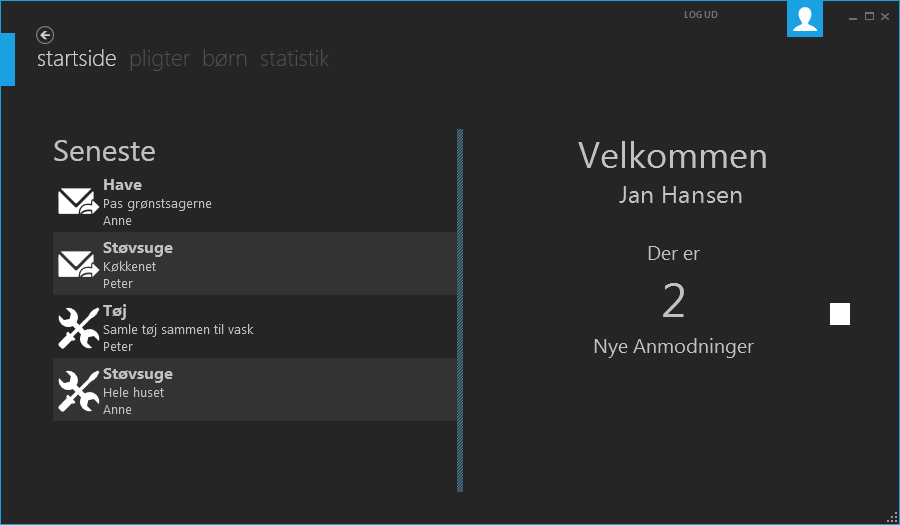
\includegraphics[width=1\textwidth]{Billeder/AdminHomeGUI.png}
\caption{Startside GUI for administrerende brugere}
\label{AdminHome}
\end{figure}

’Pligter’ fanen for administratorer var tiltænkt at skulle indeholde alle pligterne i systemet på en samlet liste placeret efter deres tilstand. Dette blev ændret til tre forskellige lister, som hver især indeholder pligter alt efter deres tilstand. Hvis der er en ledig pligt så er den i den højre liste, hvis den er påtaget så er den i den midterste, og hvis den er anmodet om at være færdig, så er den i den venstre liste. Dette blev ændret fordi det er generelt bedre, og giver et bedre og hurtigere overblik over hvilken tilstand forskellige pligter er i. Se figur \ref{AdminChore}.

\begin{figure}[H]
\centering
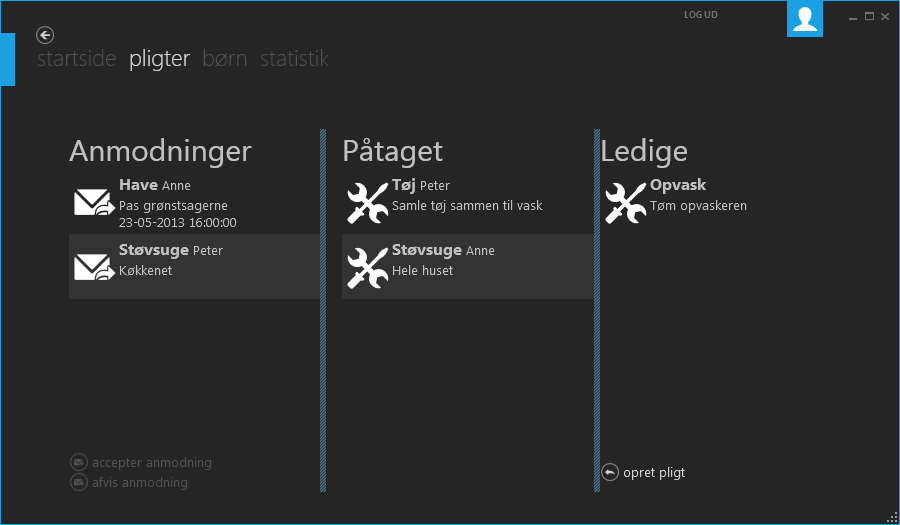
\includegraphics[width=1\textwidth]{Billeder/AdminChoreGUI.png}
\caption{Pligter GUI for administrerende brugere}
\label{AdminChore}
\end{figure}

’Statistik’ fanen for både de almindelige og administrerende brugere blev ændret i hvordan elementerne var stillet op. I Design afsnittet blev elementerne i denne fane stillet op ved siden af hinanden horisontalt. Det blev ændret til at de to grafer står ved siden af hinanden øverst på fanen, mens listen over transaktioner ligger nedenunder. Dette blev gjort fordi listen over transaktioner eller ville blive mast sammen, og der ikke ville være mulighed for at vise alle nødvendige informationer angående en transaktion. Se figur \ref{AdminStatistic}.

\begin{figure}[H]
\centering
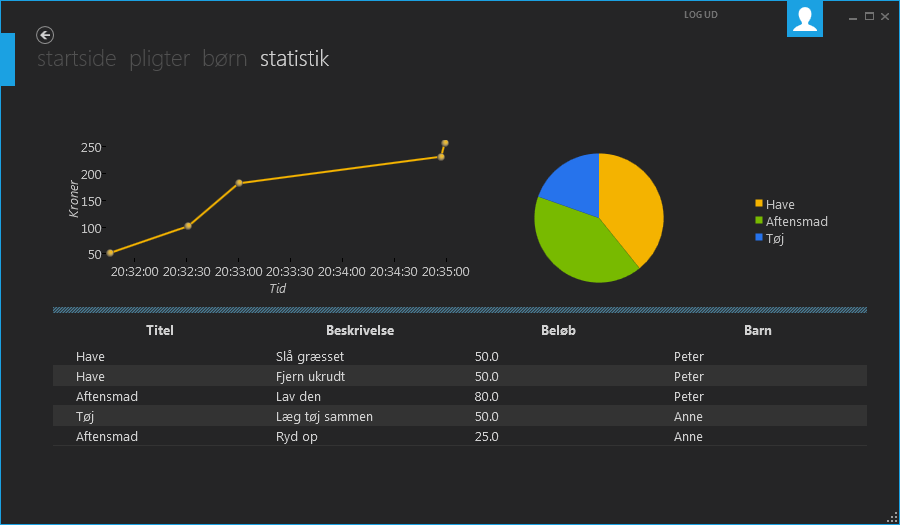
\includegraphics[width=1\textwidth]{Billeder/AdminStatisticGUI.png}
\caption{Statistik GUI for administrerende brugere}
\label{AdminStatistic}
\end{figure}